\documentclass[tikz,border=3pt]{standalone}
\usepackage[utf8]{inputenc}
\usepackage[T1]{fontenc}
\usepackage{lmodern}
\renewcommand{\familydefault}{\sfdefault}
\usepackage{sansmath}\sansmath
\usepackage{chemfig}
\usepackage{pgfplots}\pgfplotsset{compat=1.18,/pgf/number format/use comma,/pgf/number format/1000 sep={.}}
\usetikzlibrary{arrows.meta,calc,positioning,decorations.pathmorphing,patterns}
% paleta del sitio
\definecolor{nar}{HTML}{E8680C}\definecolor{narc}{HTML}{FFB35C}\definecolor{hielo}{HTML}{FFF3E8}
\definecolor{tinta}{HTML}{1D1D1F}\definecolor{gris}{HTML}{6E6E73}\definecolor{lila}{HTML}{7C5CF0}
\definecolor{azul}{HTML}{2F6FD6}\definecolor{menta}{HTML}{17A673}\definecolor{coral}{HTML}{E8342A}
\begin{document}
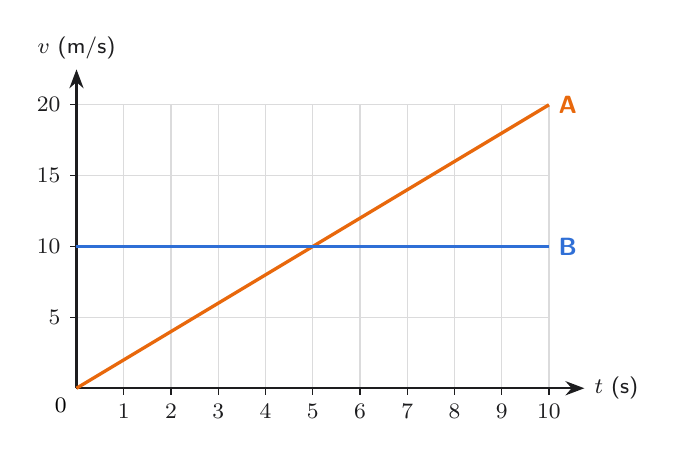
\begin{tikzpicture}[font=\footnotesize,>={Stealth[length=2.4mm]},x=0.6cm,y=0.18cm]
\draw[gris!25] (0,5) -- (10,5);
\draw[gris!25] (0,10) -- (10,10);
\draw[gris!25] (0,15) -- (10,15);
\draw[gris!25] (0,20) -- (10,20);
\draw[gris!25] (1,0) -- (1,20);
\draw[gris!25] (2,0) -- (2,20);
\draw[gris!25] (3,0) -- (3,20);
\draw[gris!25] (4,0) -- (4,20);
\draw[gris!25] (5,0) -- (5,20);
\draw[gris!25] (6,0) -- (6,20);
\draw[gris!25] (7,0) -- (7,20);
\draw[gris!25] (8,0) -- (8,20);
\draw[gris!25] (9,0) -- (9,20);
\draw[gris!25] (10,0) -- (10,20);
\draw[->,thick,tinta] (0,0) -- (10,0) -- ++(0.45cm,0) node[right] {$t$ (s)};
\draw[->,thick,tinta] (0,0) -- (0,20) -- ++(0,0.45cm) node[above] {$v$ (m/s)};
\draw[tinta] (1,0) -- ++(0,-0.08cm) node[below] {$1$};
\draw[tinta] (2,0) -- ++(0,-0.08cm) node[below] {$2$};
\draw[tinta] (3,0) -- ++(0,-0.08cm) node[below] {$3$};
\draw[tinta] (4,0) -- ++(0,-0.08cm) node[below] {$4$};
\draw[tinta] (5,0) -- ++(0,-0.08cm) node[below] {$5$};
\draw[tinta] (6,0) -- ++(0,-0.08cm) node[below] {$6$};
\draw[tinta] (7,0) -- ++(0,-0.08cm) node[below] {$7$};
\draw[tinta] (8,0) -- ++(0,-0.08cm) node[below] {$8$};
\draw[tinta] (9,0) -- ++(0,-0.08cm) node[below] {$9$};
\draw[tinta] (10,0) -- ++(0,-0.08cm) node[below] {$10$};
\draw[tinta] (0,5) -- ++(-0.08cm,0) node[left] {$5$};
\draw[tinta] (0,10) -- ++(-0.08cm,0) node[left] {$10$};
\draw[tinta] (0,15) -- ++(-0.08cm,0) node[left] {$15$};
\draw[tinta] (0,20) -- ++(-0.08cm,0) node[left] {$20$};
\node[below left] at (0,0) {$0$};
\draw[very thick,nar] (0,0) -- (10,20);
\draw[very thick,azul] (0,10) -- (10,10);
\node[right,font=\small\bfseries,text=nar] at (10,20) {A};\node[right,font=\small\bfseries,text=azul] at (10,10) {B};
\end{tikzpicture}
\end{document}
